\subsection{Gaussian Process}
\label{chap:gaussian}
In case of SLAM with physical phenomena the approximation of the underlying function is done 
with gaussian processes. A gaussian process is a stochastic process, so it consists of a set of random
variables which are index by time or space. Random variables of a gaussian process are especially multivariate
normal distributed. So every finite subset of a gaussian process is again multivariate normal distributed.

Gaussian processes are defined by a mean function $m(t)$ and a covariance function $k(x_i, x_j)$ also called kernel.
If $m(t) = 0$ the gaussian process is called centered. For the kernel radial basis function can be used. Such
gaussian processes are called radial. For a radial covariance function follows $k(x_i, x_j) = k(||x_i - x_j||)$. 
One very common radial kernel is the squared exponential kernel \cite{ebden_gaussian_2015}:

$$
k(x_i, x_j) = \sigma ^2 \exp 
\begin{pmatrix}
	-\frac{(x_i - x_j)^2}{2l^2}
\end{pmatrix}
$$

It is also possible to model noisy measurements with gaussian processes. Assume the noise is normal distributed
with variance $\sigma^2$. Then measurements can be described like $y_i = f(x_i) + \mathcal{N}(0, \sigma^2)$.
Combining the covariance function with the model of noisy measurements, that will lead to the slightly 
changed kernel:
$$
k(x_i, x_j) = \sigma ^2 \exp 
\begin{pmatrix}
	-\frac{(x_i - x_j)^2}{2l^2}
\end{pmatrix}
+ \delta_{ij} \sigma^2_{noise}
$$
In this kernel $\delta_{ij}$ is the Kronecker delta. This function is only $1$ when $i=j$ otherwise it is $0$. 
So, $\sigma^2$ is only added to the measurements. Figure \ref{fig:gaussian_process_example} gives an example 
for gaussian processes with and without noisy measurements.

Assume now there are $n$ measurements $y_1, ..., y_n$ taken at $x_1, ..., x_n$. Then the covariance matrix 
would be:
$$
K = \begin{bmatrix}
	k(x_1, x_1) & k(x_1, x_2) & \dots & k(x_1, x_n) \\
	k(x_2, x_1) & k(x_2, x_2) & \dots & k(x_2, x_n) \\
	\vdots & \vdots & \ddots & \vdots \\
	k(x_n, x_1) & k(x_n, x_2) & \dots & k(x_n, x_n) \\
\end{bmatrix}
$$
Estimating $y^*$ at $x^*$ and assuming the kernel is radial, would lead to a covariance matrix:
$$
\begin{bmatrix}
	K & K_*^T \\
	K_* & K_{**} \\
\end{bmatrix} \text{ with}
$$
$$
K_* = [k(x_*, x_1), \dots, k(x_*, x_n)],
$$
$$
K_{**} = k(x_*, x_*)
$$
Because of gaussian processes modelling data from a multivariate normal distribution, $y$ and $y_*$ 
can be modeled as:
$$
\begin{bmatrix}
	y \\
	y_* \\
\end{bmatrix} 
\sim
\mathcal{N} 
\begin{pmatrix}
	0, 
	\begin{bmatrix}
		K & K_*^T \\
		K_* & K_{**} \\
	\end{bmatrix}
\end{pmatrix}
$$
Using the mathematics of multivariate gaussian distributions, the most likely value of $y_*$ can be 
calculated by:
\newpage
$$
y_*|y \sim \mathcal{N}(K_*K^{-1}y, K_{**} - K_*K^{-1}K_*^T)
$$
$$
\Rightarrow \bar{y}_* = K_*K^{-1}y
$$
The derivation of the formula is well explained by Ebden in 2008 \cite{ebden_gaussian_2015}. Notice that
also the variance for $y_*$ is given by:
$$
var(y_*) = K_{**} - K_*K^{-1}K_*^T
$$

All that, uncertainty in measurements, prediction of $y_*$ and probability of the prediction can be seen
in figure \ref{fig:gaussian_process_example}. Note that for linear increasing measurements the size of the 
covariance matrix rises quadratically and for $y_*$ the inverse of that matrix has to be calculated. 
So it is quite slow for large scale data. Some approaches facing that will be described in the next chapter.
Another remark is that the standard gaussian process is not possible to model uncertainty in the input data.
A recent approach for that will also be presented in the chapter \ref{chap:uncertain_inputs}. 

\begin{figure}[h!]
	\centering
	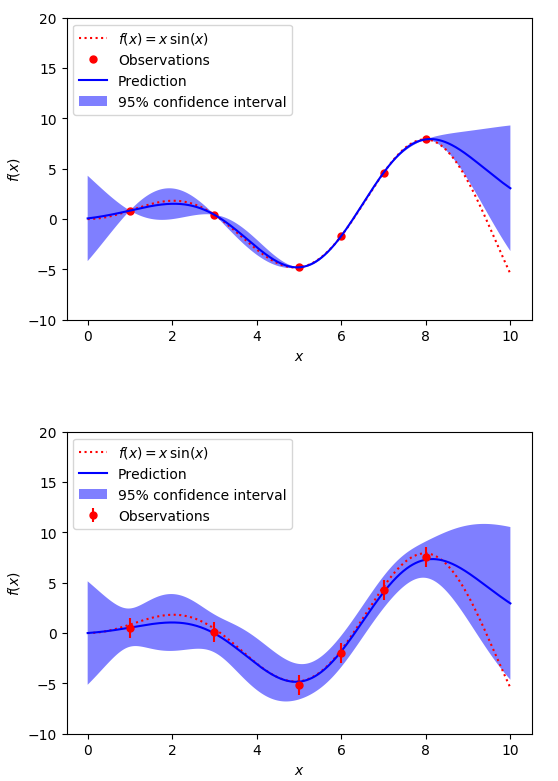
\includegraphics[width=0.425\textwidth]{images/gaussian_process_example.png}
	\caption{
			Plot of two gaussian processes regressions with the same measurement points $x_i$
			but the one at the bottom has noisy measurements with variance $\sigma_{noise}^2 = 1$.
			Also noticeable the probability of the predictions represented through the confidence interval.
        }
	\label{fig:gaussian_process_example}
\end{figure}

